\documentclass[IN,english]{tumbook}
\usepackage{tabularx}
%\usepackage[utf8]{inputenc}
%\usepackage[T1]{fontenc}
%\usepackage{graphicx}
%\usepackage{amsmath}

\makeindex

% Information for the title page
\Seminar{Software Engineering for Business Applications - Master}
\Semester{SS 2015}
\title{Mockups for the Web Application \emph{Travel Diary}}
\Untertitel{}
\Themensteller{Prof. Dr. Florian Matthes}
\Autorenadresse{}
\Matrikelnummer{}
\Fachsemester{}
\Abgabetermin{13. May 2015}
\author{Chetan Basuray, Mantosh Kumar, Ulrike Niemann, Albert Steckermeier}
\date{13. May 2015}



\begin{document}

\maketitle
\newpage
\tableofcontents
\newpage

\chapter{Use Case 1: Searching for Vacations}

\chapter{Use Case 2: Sharing the Experience of an Activity}

\chapter{Use Case 3: Sharing the Experience of a Vacation}

\chapter{Use Case 4: Planning a Vacation}

Figure \ref{fig:usecase4} shows the vacation view. Here all the activities of the vacation \emph{Trip to Munich} are shown. The pin icon at the top left of an activity allows the user to move the activities around. Activities can be deleted by clicking the red trash icon in the top right corner. In the vacation view the search bar at the top automatically searches for activities instead of vacations. A new activity is added by searching it via the search bar and adding it by clicking an add button which will replace the trash icon in the search results for new activities.

\begin{figure}
	\begin{center}
		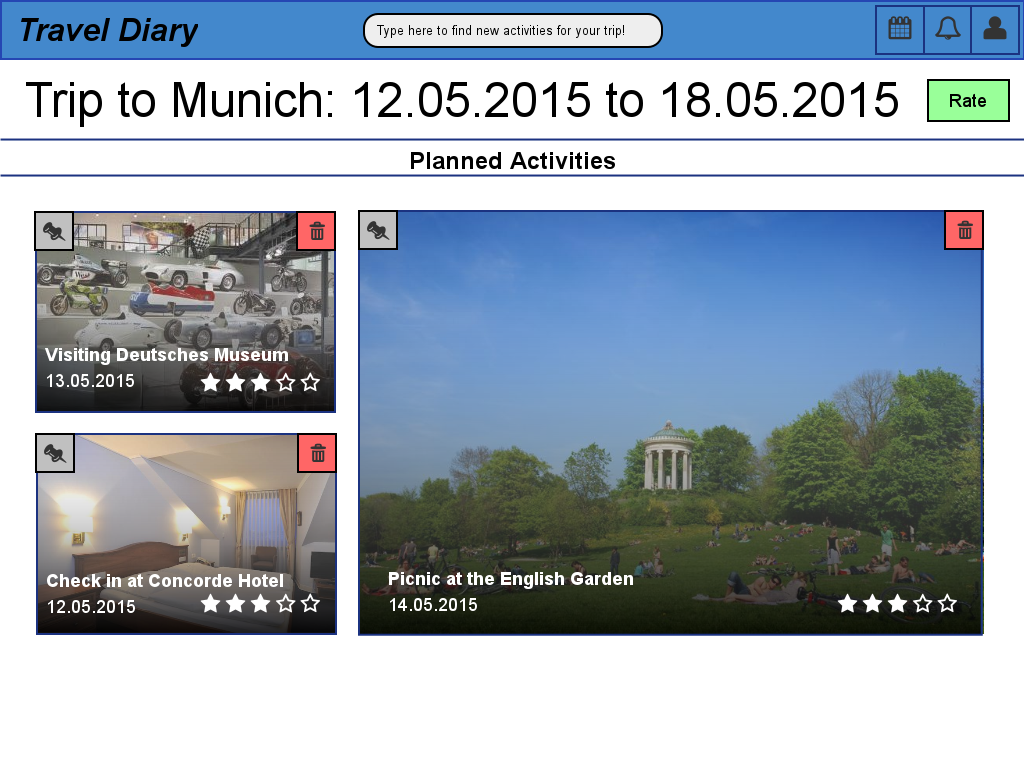
\includegraphics[scale=0.5]{graphics/usecase4}
	\end{center}
	\label{fig:usecase4}
	\caption{A mockup for the vacation view of \emph{Travel Diary}.}
\end{figure}

\end{document}